\documentclass[paper=letter,11pt]{scrartcl}

\KOMAoptions{headinclude=true, footinclude=false}
\KOMAoptions{DIV=14, BCOR=5mm}
\KOMAoptions{numbers=noendperiod}
\KOMAoptions{parskip=half}
\addtokomafont{disposition}{\rmfamily}
\addtokomafont{part}{\LARGE}
\addtokomafont{descriptionlabel}{\rmfamily}
%\setkomafont{pageheadfoot}{\normalsize\sffamily}
\setkomafont{pagehead}{\normalsize\rmfamily}
%\setkomafont{publishers}{\normalsize\rmfamily}
\setkomafont{caption}{\normalfont\small}
\setcapindent{0pt}
\deffootnote[1em]{1em}{1em}{\textsuperscript{\thefootnotemark}\ }


\usepackage{amsmath}
\usepackage[varg]{txfonts}
\usepackage[T1]{fontenc}
\usepackage{graphicx}
\usepackage{xcolor}
\usepackage[american]{babel}
% hyperref is needed in many places, so include it here
\usepackage{hyperref}

\usepackage{xspace}
\usepackage{multirow}
\usepackage{float}


\usepackage{braket}
\usepackage{bbm}
\usepackage{relsize}
\usepackage{tcolorbox}

\def\ketY{\ensuremath{\ket {\Psi}}}
\def\iGeV{\ensuremath{\textrm{GeV}^{-1}}}
%\def\mp{\ensuremath{m_{\textrm{proton}}}}
\def\rp{\ensuremath{r_{\textrm{proton}}}}
\def\me{\ensuremath{m_{\textrm{electron}}}}
\def\aG{\ensuremath{\alpha_G}}
\def\rAtom{\ensuremath{r_{\textrm{atom}}}}
\def\rNucl{\ensuremath{r_{\textrm{nucleus}}}}
\def\GN{\ensuremath{\textrm{G}_\textrm{N}}}
\def\ketX{\ensuremath{\ket{\vec{x}}}}
\def\ve{\ensuremath{\vec{\epsilon}}}


\def\ABCDMatrix{\ensuremath{\begin{pmatrix} A &  B  \\ C  & D \end{pmatrix}}}
\def\xyprime{\ensuremath{\begin{pmatrix} x' \\ y' \end{pmatrix}}}
\def\xyprimeT{\ensuremath{\begin{pmatrix} x' &  y' \end{pmatrix}}}
\def\xy{\ensuremath{\begin{pmatrix} x \\ y \end{pmatrix}}}
\def\xyT{\ensuremath{\begin{pmatrix} x & y \end{pmatrix}}}

\def\IMatrix{\ensuremath{\begin{pmatrix} 0 &  1  \\ -1  & 0 \end{pmatrix}}}
\def\IBoostMatrix{\ensuremath{\begin{pmatrix} 0 &  1  \\ 1  & 0 \end{pmatrix}}}
\def\JThree{\ensuremath{\begin{pmatrix}    0 & -i & 0  \\ i & 0  & 0 \\ 0 & 0 & 0 \end{pmatrix}}} 
\def\JTwo{\ensuremath{\begin{bmatrix}    0 & 0 & -i  \\ 0 & 0  & 0 \\ i & 0 & 0 \end{bmatrix}}}
\def\JOne{\ensuremath{\begin{bmatrix}    0 & 0 & 0  \\ 0 & 0  & -i \\ 0 & i & 0 \end{bmatrix}}}
\def\etamn{\ensuremath{\eta_{\mu\nu}}}
\def\Lmn{\ensuremath{\Lambda^\mu_\nu}}
\def\dmn{\ensuremath{\delta^\mu_\nu}}
\def\wmn{\ensuremath{\omega^\mu_\nu}}
\def\be{\begin{equation*}}
\def\ee{\end{equation*}}
\def\bea{\begin{eqnarray*}}
\def\eea{\end{eqnarray*}}
\def\bi{\begin{itemize}}
\def\ei{\end{itemize}}
\def\fmn{\ensuremath{F_{\mu\nu}}}
\def\fMN{\ensuremath{F^{\mu\nu}}}
\def\bc{\begin{center}}
\def\ec{\end{center}}
\def\nus{$\nu$s}

\def\adagger{\ensuremath{a_{p\sigma}^\dagger}}
\def\lineacross{\noindent\rule{\textwidth}{1pt}}

\newcommand{\multiline}[1] {
\begin{tabular} {|l}
#1
\end{tabular}
}

\newcommand{\multilineNoLine}[1] {
\begin{tabular} {l}
#1
\end{tabular}
}



\newcommand{\lineTwo}[2] {
\begin{tabular} {|l}
#1 \\
#2
\end{tabular}
}

\newcommand{\rmt}[1] {
\textrm{#1}
}


%
% Units
%
\def\m{\ensuremath{\rmt{m}}}
\def\GeV{\ensuremath{\rmt{GeV}}}
\def\pt{\ensuremath{p_\rmt{T}}}


\def\parity{\ensuremath{\mathcal{P}}}

\usepackage{cancel}
\usepackage{ mathrsfs }
\def\bigL{\ensuremath{\mathscr{L}}}

\usepackage{ dsfont }



\usepackage{fancyhdr}
\fancyhf{}

%\documentclass[margin,line]{res}
\usepackage{braket}
\usepackage{bbm}
\usepackage{relsize}

\def\ketY{\ensuremath{\ket {\Psi}}}
\def\iGeV{\ensuremath{\textrm{GeV}^{-1}}}


\def\ABCDMatrix{\ensuremath{\begin{pmatrix} A &  B  \\ C  & D \end{pmatrix}}}
\def\xyprime{\ensuremath{\begin{pmatrix} x' \\ y' \end{pmatrix}}}
\def\xyprimeT{\ensuremath{\begin{pmatrix} x' &  y' \end{pmatrix}}}
\def\xy{\ensuremath{\begin{pmatrix} x \\ y \end{pmatrix}}}
\def\xyT{\ensuremath{\begin{pmatrix} x & y \end{pmatrix}}}

\def\IMatrix{\ensuremath{\begin{pmatrix} 0 &  1  \\ -1  & 0 \end{pmatrix}}}
\def\IBoostMatrix{\ensuremath{\begin{pmatrix} 0 &  1  \\ 1  & 0 \end{pmatrix}}}
\def\JThree{\ensuremath{\begin{pmatrix}    0 & -i & 0  \\ i & 0  & 0 \\ 0 & 0 & 0 \end{pmatrix}}} 
\def\JTwo{\ensuremath{\begin{bmatrix}    0 & 0 & -i  \\ 0 & 0  & 0 \\ i & 0 & 0 \end{bmatrix}}}
\def\JOne{\ensuremath{\begin{bmatrix}    0 & 0 & 0  \\ 0 & 0  & -i \\ 0 & i & 0 \end{bmatrix}}}
\def\etamn{\ensuremath{\eta_{\mu\nu}}}
\def\Lmn{\ensuremath{\Lambda^\mu_\nu}}
\def\dmn{\ensuremath{\delta^\mu_\nu}}
\def\wmn{\ensuremath{\omega^\mu_\nu}}
\def\be{\begin{equation*}}
\def\ee{\end{equation*}}
\def\bc{\begin{center}}
\def\ec{\end{center}}
\def\nus{$\nu$s}
%\def\xMu{\ensuremath{x^\mu}

\usepackage{fancyhdr}

\fancyhf{}
\lhead{\Large 33-444} % \hfill Introduction to Particle Physics \hfill Spring 2020}
\chead{\Large Introduction to Particle Physics} % \hfill Spring 2020}
\rhead{\Large Spring 2020} % \hfill Introduction to Particle Physics \hfill Spring 2020}

\begin{document}
\thispagestyle{fancy}

\begin{center}
{\huge \textbf{Lecture 34}}
\end{center}

{\fontsize{14}{16}\selectfont

\textbf{\underline{OK left off discussing solar \nus}} 

\underline{Bottom line}: Solar fusion takes lighter nuclei and might bigger ones.  
This creates \nus\ (not anti-\nus\ like $\beta$ decay)

We also talked about how you can calculate the neutrino flux from the sun and the expected energy spectrum.
Here's what you get:

\begin{figure}[h!]
\centering
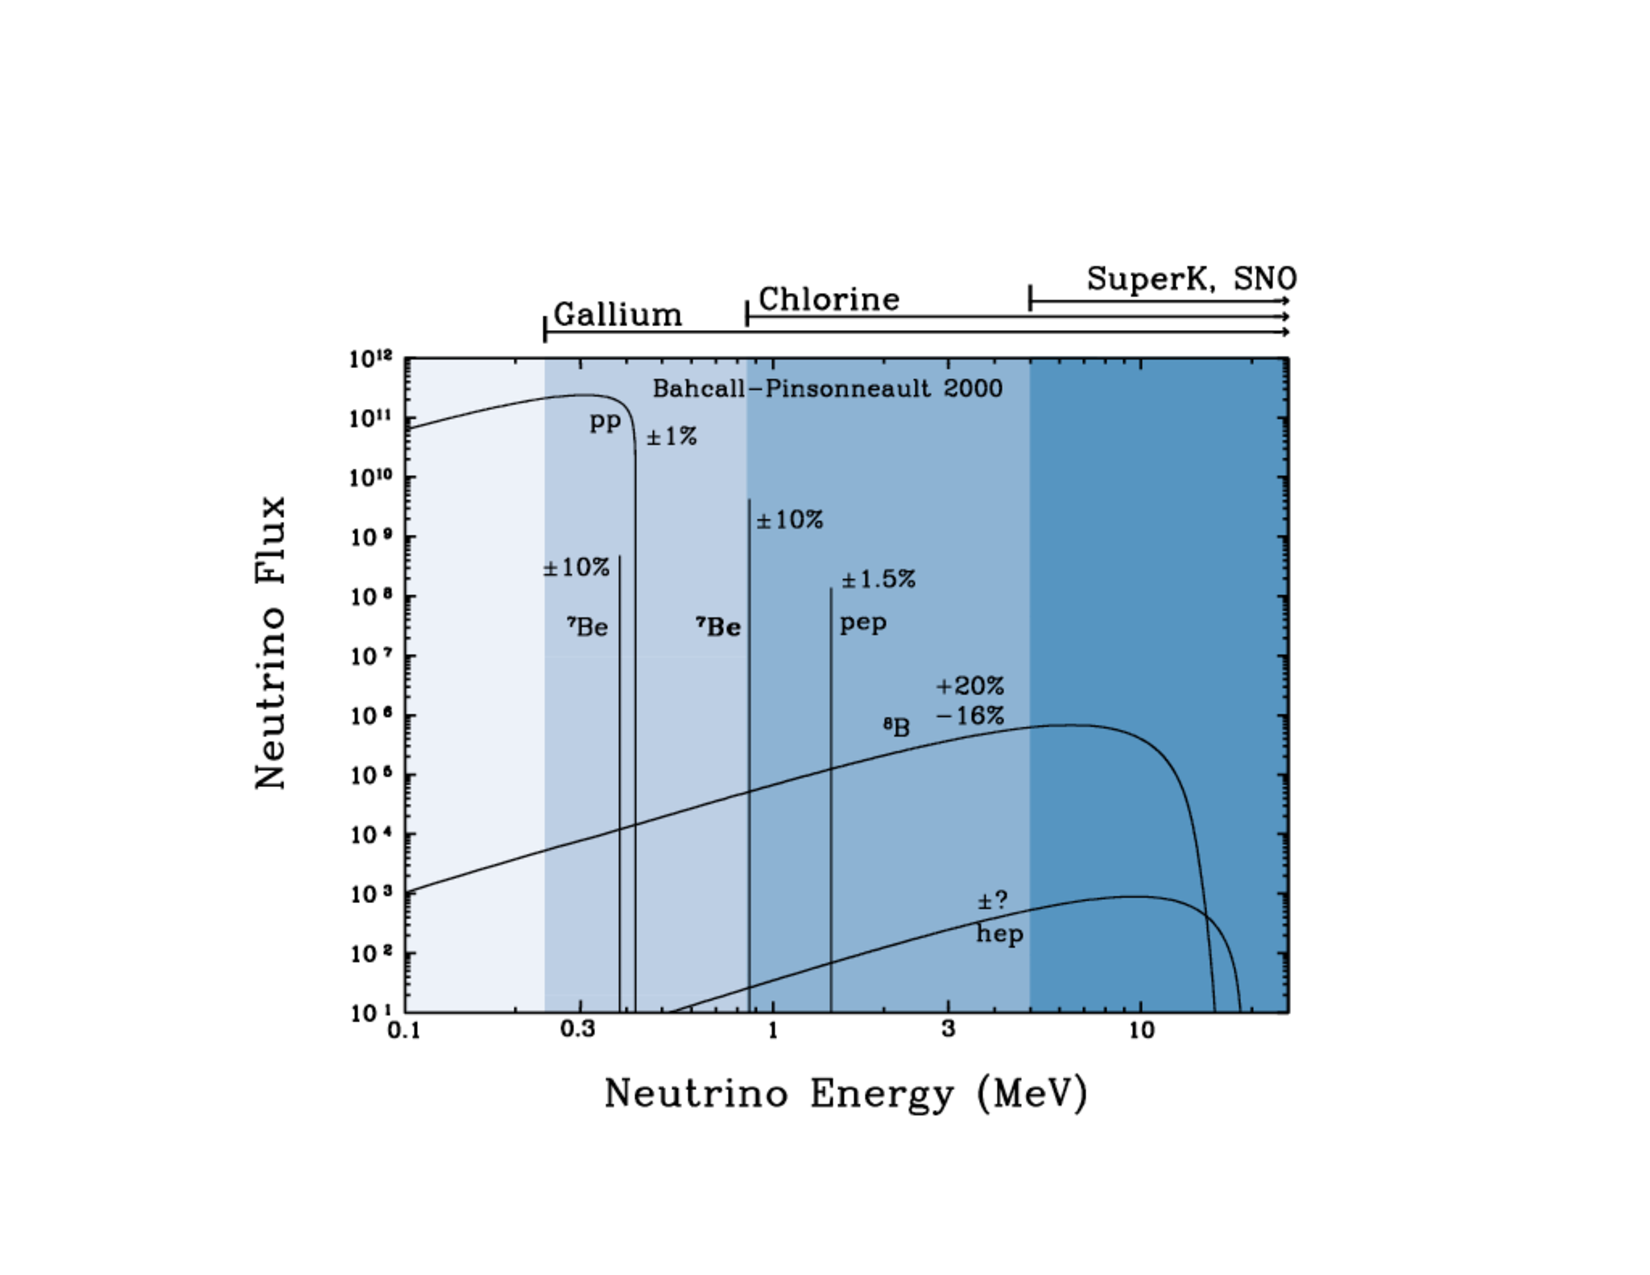
\includegraphics[width=1.0\textwidth]{./NuFromSun.pdf}
\end{figure}

Most of the \nus\ are relatively low energy (below 1 MeV) ``low energy \nus''
How do we detect? these low energy \nus ?

We've developed several different way to do this. 
The oldest one was an experiment that started in the 60s using Chlorine. 
Remember the cross sections are incredibly small, so you need a large amount of something that is going to be your target. 

Now you would like to them see them by having them hit something, but they only interact via W or Z. 
If interact via Z, at these really low energies the best you can get is that if the $\nu$ hits something it will make that something recoil. 
This is very challenging to observe.  
We have actually only just recently (within last year or so) observed this process. 
(Ironically this will likely be the biggest background for DM detection in the future, but we will come back to this later in the course) 

The other process you can look for is that a $\nu$ interacts with via charged current and it will produce an electron. 
Now you are sort of in business b/c you have an electron, but the big challenge is you live in a big complicated environments.
And you have to get a signal from a low energy electron (b/c the \nus\ are low energy).

The ideas that people had for how to measure these \nus\ in the beginning were different than standard ways that particle physicists would think about doing experiments. 
First one was a chlorine experiment.  
Here you are looking for the following reaction:
\be
\nu_e + Cl \rightarrow e^- + Ar
\ee
And the idea is that you have a really big detector made out of chlorine; the \nus\ produce Ar and your are going to see this Ar. 
Great idea b/c Ar is a noble gas (wont mix with environment), so if you have a way of separating Ar and Cl you're in good shape. 
Actually better than, this bc you make the Ar in an excited state that has a fairly long lifetime. 
So you can get the Ar* out the detector and look for Ars decaying. (Very clever idea). 

Turns out you can actually do the same thing with Gallium and Germanium. 

There are Very very very hard experiments!
Just from the shear numbers that you have to work with. 

Famous experiment ``Ray Davis experiment.''
Cl is easy to get, buy it in bulk in the store (basically cleaning liquid)
Put it a gigantic vat, wait for a month, and the signal is a handful of atoms/month in a massive tank of Cl. 
Think tanker-truck of Cl, and you're looking for a \textbf{few atoms} every month.
Very hard and very unusual for particle physics people.
It actually mostly involves a lot of chemistry (And as we all know chemistry is very hard).

Ray Davis made this measurement for about 40 years. 
And what he found was very exciting. 
First of all he actually saw \nus\ coming from the sun!
But most importantly for us, saw fewer \nus\ that expected and not by a little bit: only saw 1/3 of \nus\ expected. 

Now historically, most people did not care about this at all.
For several reasons, 
1) doing a really hard experiment, he correct to within factor of 3. That's a great result! be happy. 
2) calculations to know what to expect are also very hard 

\noindent\rule{\textwidth}{1pt}

\textbf{Things started changing qualitatively when the very large water detectors starting coming into the game. }

They chose to measure something else.
For a $\nu$ interacting in water there are three potential targets:  O, H, electrons.

1) Turns out oxygen is very unhappy to be hit by a $\nu$ and give an electron. 
Oxygen is a very stable nucleus, very tightly bound.

2) \nus\ have a hard time hitting protons b/c of lepton number conservation. 
They would have to produce electrons (b/c they have electron flavour +1). 
However, the proton already has +charge.  
So the proton would have to turn into something with doubly-plus charge which is not possible at low energies. 

So in the big water detectors the things you can hit are the electrons. 
\be
\nu + e \rightarrow \nu + e
\ee

This is a very interesting process.
Turns out that in these very big water tanks (that were by the way constructed originally to see proton decay, \textit{more on this later in the course}) we could see electrons.
Even relatively low electrons, MeV-type electrons with Cerenkov radiation that you read all about on last homework.

These started coming online in the late 80s/early 90s.

\noindent\rule{\textwidth}{1pt}

\textbf{(Side note.)}
Actually the Chlorine detector that discovered the solar \nus, the first thing they did was put it next to a nuclear reactor.
Remember these are strong source of anti-\nus.
Curiously enough, they didn't see anything.
This is actually a big deal, (they knew they weren't supposed to see anything, the reactor is emitting anti-\nus\ not \nus) 
And the the Chlorine reaction doesn't work with anti-\nus. 

It is interesting they didn't see anything, confirms prediction. 
Now, this this was done in US, and there was actually a rumor that they did see something which peculated to Europe and then to soviet union. 
Pontecorvo, who was in exile in the USSR came up with a model of hoe a $\nu$ can behave like an anti-nu.
This was a model of $\nu$/ $anti-\nu$ oscillations. 
This was a model that was invented for a false rumor! 
And as will see it eventually morphed into the $\nu$ oscillations that we know today (among flavours). 

\noindent\rule{\textwidth}{1pt}

OK anyway, here are the results of the measurements of solar \nus.


\begin{figure}[h!]
\centering
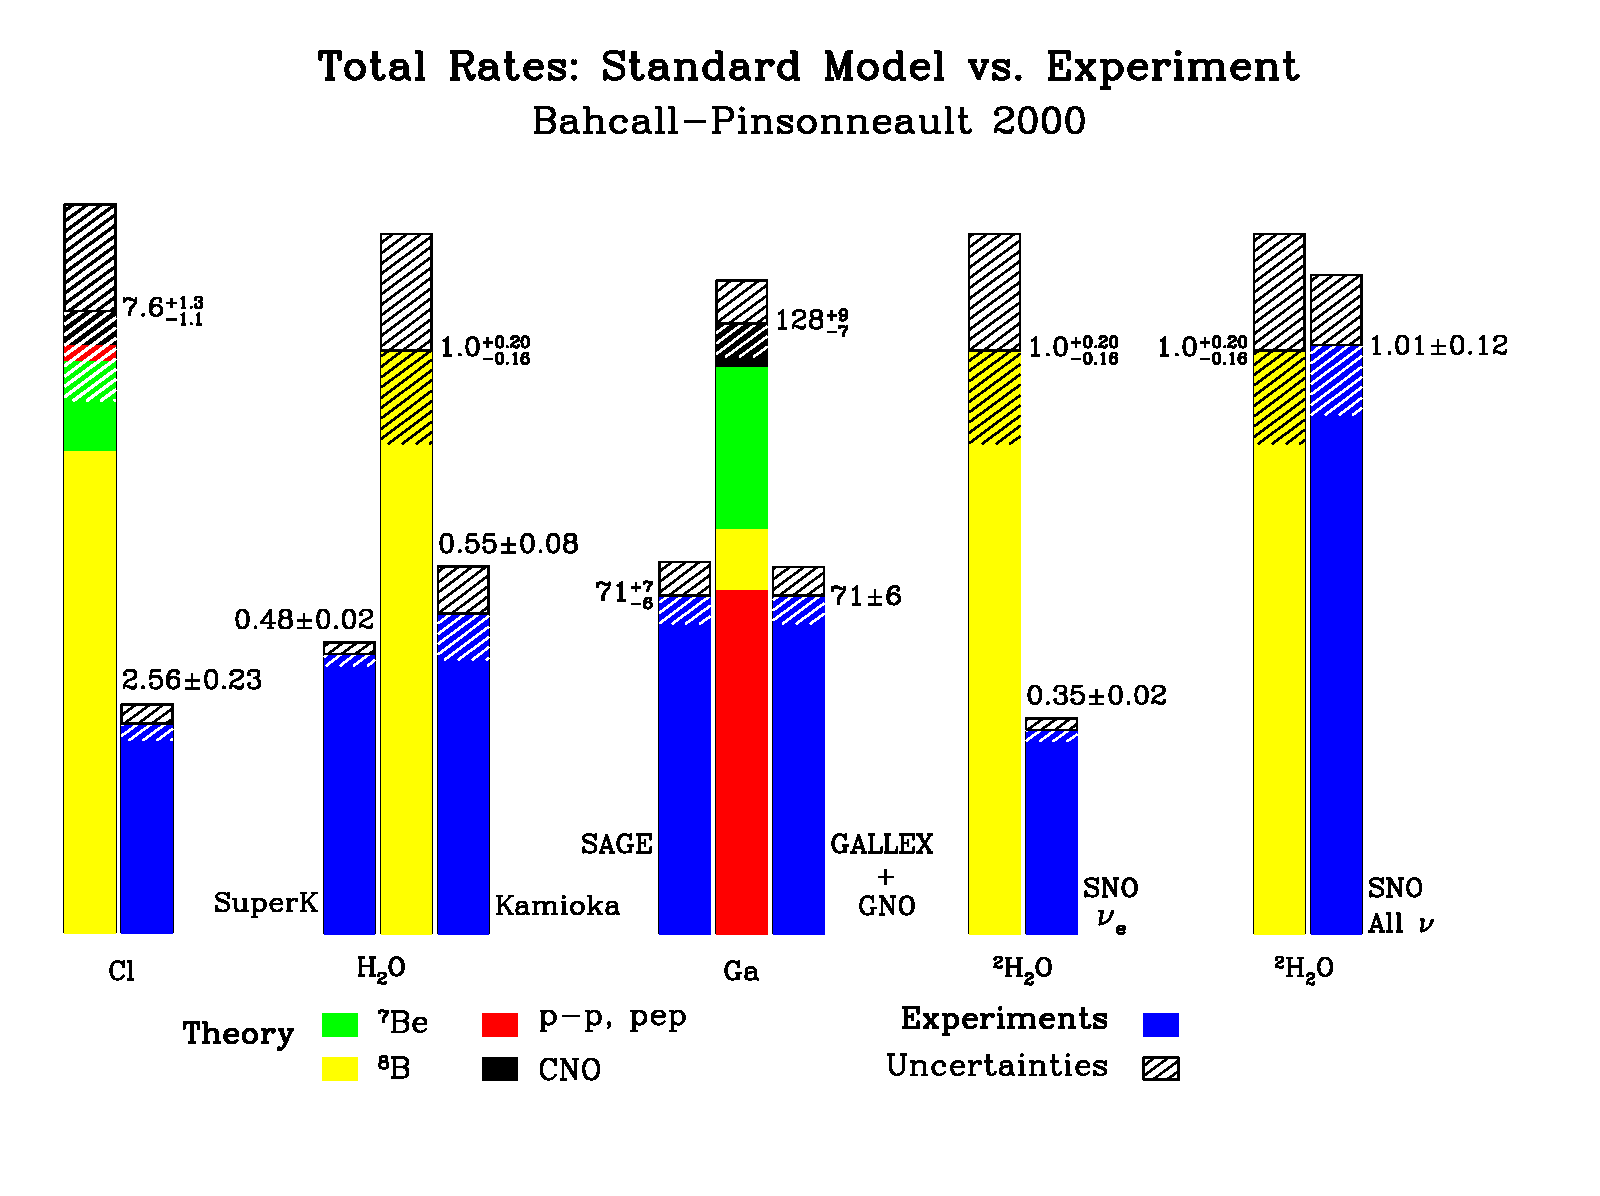
\includegraphics[width=1.0\textwidth]{./SolarNuPuzzle.pdf}
\end{figure}


This is a complicated plot. 
The colored (non-blue) bars are the expectations for what you should see.
And the blue measurements are how many \nus\ where actually observed.  
If you ignore the right-hand bars for a second, the rest of the picture is what is called the ``solar neutrino puzzle''. 
Seeing fewer \nus\ that we expected. 
A bunch of different experiments were performed..  
So that maybe if you didn't believe the initial Cl experiment, there were all these other experiments that were still seeing a deficit. 

Lots of logical possibilities for whats going wrong. 

1) all making a coherent mistake, but this is why we do lots of experiments.  Very unlikely that they all can be going wrong. 

2) our understanding of the sun is not as good as we thought it was.
(Turns out, for detailed reasons I wont go into, we knew  that the solar model wasn't wrong at the level we needed to explain the data

3) (last hypothesis) or our understanding of how \nus\ propagate is wrong. 

For this last option there are a lot of things you could think about. \\
 -) Maybe \nus\ decay...\\
 -) Maybe they get absorbed, \\
 -) One hypothesis people raised was the flavour changing hypothesis\\

\noindent\rule{\textwidth}{1pt}

\textbf{Flavour Changing Neutrinos}

Very simple hypothesis, we will come back to the mechanism in detail later. 
Basic idea, even if the sun can only produce electron \nus, by the time they get to earth some of them have turned into $\mu$ or $\tau$ \nus. 


This hypothesis can actually explain all of the measurements.  

All of the experiments are only (mainly) sensitive to electron \nus.

\bc
$\nu_e + e \rightarrow \nu_e + e$  (has both neutral and charged currents) 
\ec

\bc
$\nu_{\mu,\tau} + e \rightarrow \nu_{\mu,\tau} + e$  (only has neutral currents), 
\ec

Turns out the $\nu_{\mu,\tau} + e$ cross section is only about half that of $\nu_e + e$.

So now we actually have an opportunity to test this hypothesis, this is what the SNO experiment was about.

\noindent\rule{\textwidth}{1pt}

\clearpage

\textbf{SNO experiment}

Heavy water experiment.

Idea is if you have a way of testing the $\nu$ neutral current interaction, this process wouldn't care weather you have electron, muon or tau neutrino. 
They would all contribute in the same way. 

What they did was construct a very big tank of heavy water and they figured out for dueterons, (D  = n+p bound state), you could get the reaction
\be
\nu + D \rightarrow \nu + p + n
\ee

D is a very loosely bound bound state. (Its bizarre, ``fine tuned'' and this fact turns out to be very important for big-bang nuclear synthesis. )

So there is a possibility that the neutrino can break up the Deuteron, and this effect should happen for all three types of \nus.

OK so the idea is to do an experiment with large amount of D, if you have a way of detecting neutrons you are in business.

This is what the SNO experiment was about. 

At the same time, they could of course see the standard charged-current interaction:
\be
\nu_e + D \rightarrow e^- + p + p
\ee
(by the way detecting low-energy protons is absolutely hopeless)


Finally,  the last thing they could look for is:
\be
\nu_{e,\mu,\tau} + e  \rightarrow \nu_{e,\mu,\tau} +e
\ee
and as we said before here all the \nus\ participate, but the electron cross section is larger.

SNO was very good at looking for electrons. and they could also see neutrons

So, the same experiment can do 3 measurements at once:\\
 -) reaction where only the electron participates\\
 -) reaction where the electron participates with big cross section, and the other flavours participate with much smaller $\sigma$\\
 -) And then they see another where they all participate with the same cross section. 


So if somehow there were \nus\ arriving from the sun behaving as $\nu_\mu$s or $\nu_\tau$s, this experiment could test it. 

And that is what you see on the right hand bar bar above. 

Here is More impressive plot: 

\begin{figure}[h!]
\centering
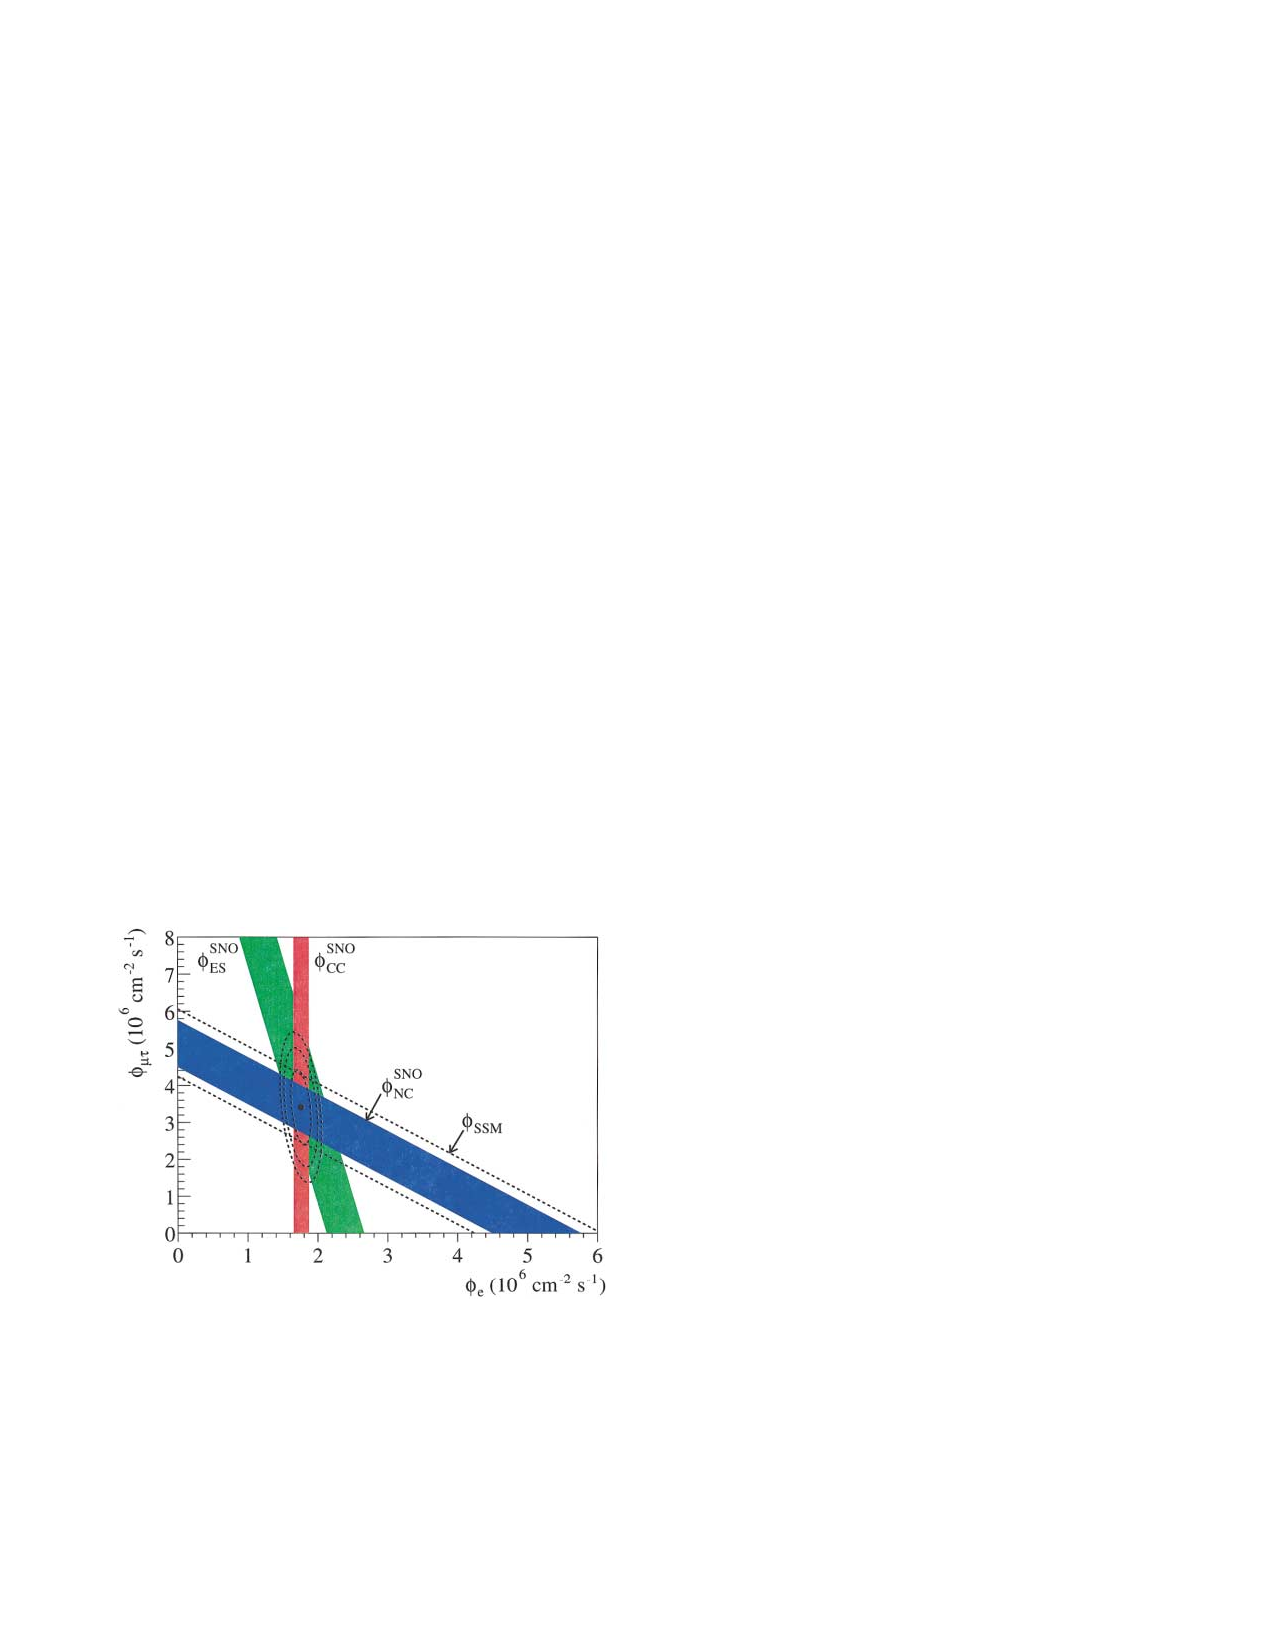
\includegraphics[width=1.0\textwidth]{./SNOResult.pdf}
\end{figure}

The x-axis is the electrons \nus\ coming from the sun. 
The y-axis is the $\mu$ or $\tau$ \nus\ coming from the sun, keep in mind the sun cannot produce these.
But by the time they get here we see them. 

The red-band is the charged current interaction that is only sensitive to electron flux. 
\be
\nu_e + D \rightarrow e^- + p + p
\ee 

The green band is the scattering is the scattering off of electrons.
This is sensitive to all three \nus, but where $\nu_e$s dominate.
\be
\nu_{e,\mu,\tau} + e  \rightarrow \nu_{e,\mu,\tau} +e
\ee
So this is also mostly a measurement of the electron flux, but there is a non-trivial contribution from the flux of the other \nus. 
So it gives you a line on this plot that has some angle to it. 
(The green error bar is bigger than the red by the cross section to hit an electron is smaller than that to hit a nuclei) 

And finally, the last result is the blue line from the neutral current interaction. 

All three lines meet at a point, which is already non-trivial statement. 
And in fact that meet at a point that agrees with our solar model. (dashed lines) 

Turns out that 2/3 of the \nus, coming from the sun are of the $\mu$ or $\tau$ flavor.
Very unambiguous result.
We know that this is happening.

In fact, red and green already tell most of the story. 
These measurements are the ``easy'' ones. 
The blue line is the measurement that involves seeing the neutrons. 
This is much harder. 
SNO actually used three different ways to detect neutrons and they all give consistent results. 

That's the experimental situation. 

So we know it's possible to produce a lot of \nus\ in the sun, and by the time they get here they are muon or tau neutrinos.

\noindent\rule{\textwidth}{1pt}

\textbf{\nus\ from the atmosphere.}

Lets now start talk now about a different experiment. 

(This is a really big deal, b/c this result became unambiguous before the SNO results came out.)

The idea here is very simple. 

When cosmic rays hit the atmosphere, you make a bunch of pions.  (If you have enough time the muons also decay) 

\be
\pi^- \rightarrow \mu^- + \bar{\nu}_\mu \rightarrow e^- + \bar{\nu_e} + \nu_\mu
\ee

So cosmic rays hitting the atmosphere are producing \nus\ all the time.  
Muon \nus\ and electron \nus. 
And these are \nus\ you can try to measure. 

Now you can make lots of predictions (eg: Total flux/ energy distribution of \nus\ / ect)
Turns out these are all ``dirty'' calculation,  depend on many unknowns. (Depend on the atmospheric conditions/depend on strong interactions) 
Its hard, but there are some robust predictions you can make. 

One of these, is that at low energies the $\mu$s don't have much energy and so they can decay. 
Then you would expect to get 2 muons type \nus\ for each electron type $\nu$. 
That's a pretty robust prediction. 

Another prediction is that the flux from below and above is the same (this is an artifact of 3D) 
Only assumption is that the flux of cosmic rays is $\sim$isotropic.

So there are two robust predictions that you can measure muon vs electron ratio and top vs down ratio. 

Will pick up here next time...

 




}
\end{document}


